\newcommand{\fix}[1]{\textcolor{red}{\texttt{#1}}} % command for comments 
%\newcommand{\fix}[1]{} % remove all comments

\chapter{Detector and Physics Performance}

\section{System performance}
\writer{Frank Gaede}{5}
\subsection{Vertexing}
\subsection{Tracking}

\fix{Tracking Efficiency plots need to be redone with pair-bg overlaid !}

%
% tracking resolution for single muons
% 
\thisfloatsetup{floatwidth=\SfigwFull,capposition=beside}
\begin{figure}[b!]
\begin{tabular}{cc}
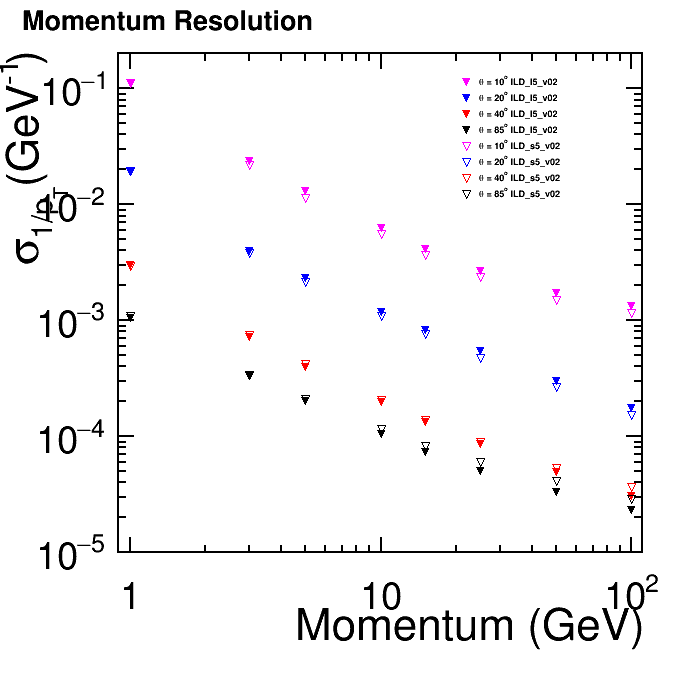
\includegraphics[width=0.5\hsize]{Performance/fig/PResolution_ILD_ls5_v02.png} &
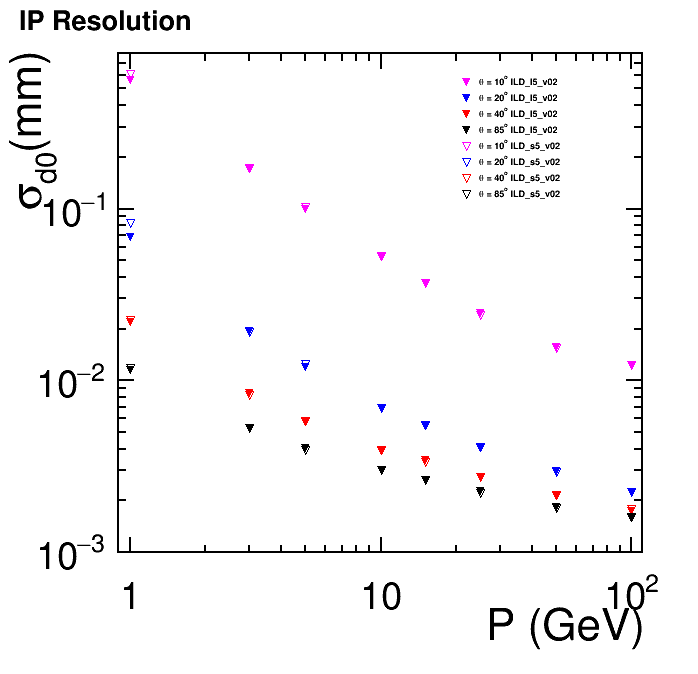
\includegraphics[width=0.5\hsize]{Performance/fig/IPResolution_ILD_ls5_v02.png}
\end{tabular}
\caption{\label{ild:fig:intro:tracking} Momentum (left) and impact parameter (right) resolution for the two ILD detector models,
  as a function of momentum of the single muon. Large detector: closed symbols - small detector: open symbols.}
\end{figure}


%
% tracking efficiency for ttbar - 1D
% 
\thisfloatsetup{floatwidth=\SfigwFull,capposition=beside}
\begin{figure}[b!]
\begin{tabular}{cc}
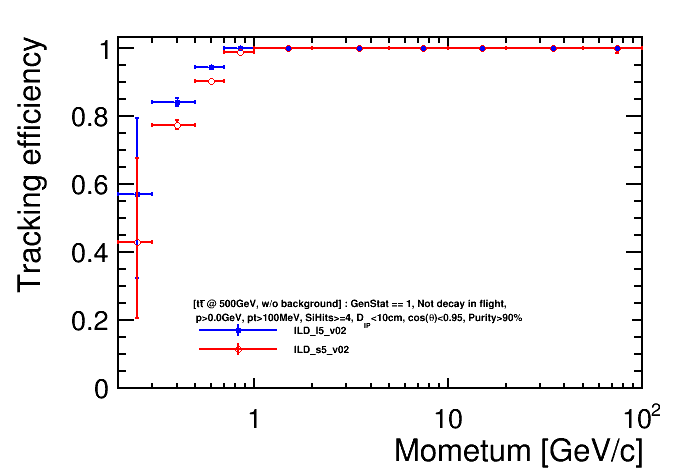
\includegraphics[width=0.5\hsize]{{Performance/fig/trkEff_Momentum_ttbar_ILD_ls5_v02_publish2}.png} &
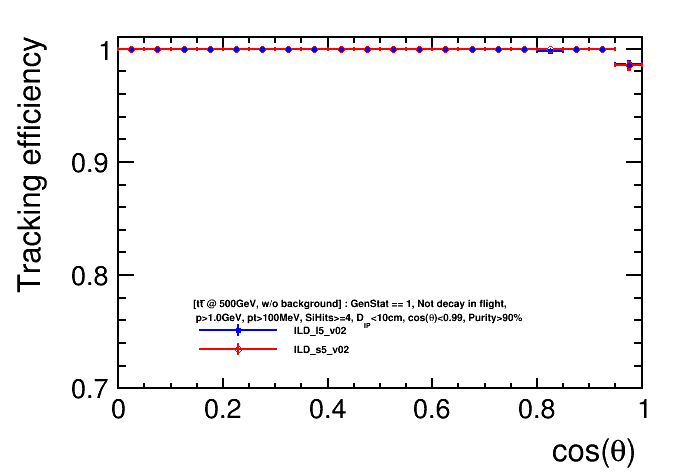
\includegraphics[width=0.5\hsize]{{Performance/fig/trkEff_theta_ttbar_ILD_ls5_v02_publish1}.png}
\end{tabular}
\caption{\label{ild:fig:intro:tracking}Track finding efficiency for $t \bar t$-events at 500 GeV, as a function of momentum (left) and 
 $cos(\theta)$ (right) for the large (red) and small (blue) ILD detector models. }
\end{figure}


%
% tracking efficiency for ttbar - as function of pt
% 
\thisfloatsetup{floatwidth=\SfigwFull,capposition=beside}
\begin{figure}[b!]
\begin{tabular}{cc}
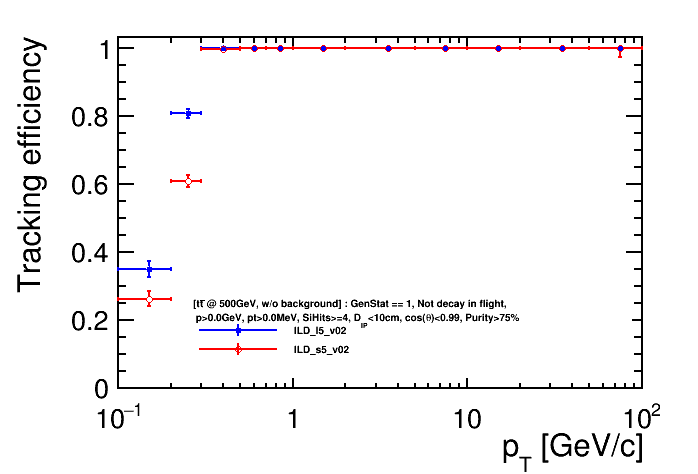
\includegraphics[width=0.5\hsize]{{Performance/fig/trkEff_pt_ttbar_ILD_ls5_v02_monitor}.png} &
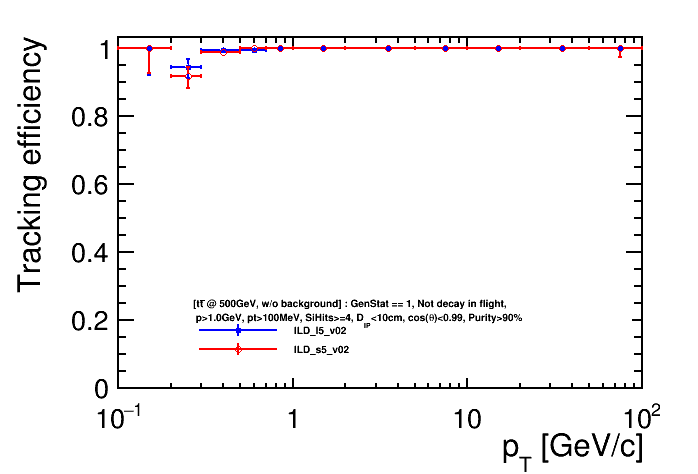
\includegraphics[width=0.5\hsize]{{Performance/fig/trkEff_pt_ttbar_ILD_ls5_v02_publish1}.png}
\end{tabular}
\caption{\label{ild:fig:intro:tracking}Track finding efficiency for $t \bar t$-events at 500 GeV, as a function of transeverse momentum for the large (red)
  and small (blue) ILD detector models. left: $p > 0 GeV$ ; right: $p > 1 GeV$ }
\end{figure}


%
% tracking efficiency for ttbar - 2D
% 
\thisfloatsetup{floatwidth=\SfigwFull,capposition=beside}
\begin{figure}[b!]
\begin{tabular}{cc}
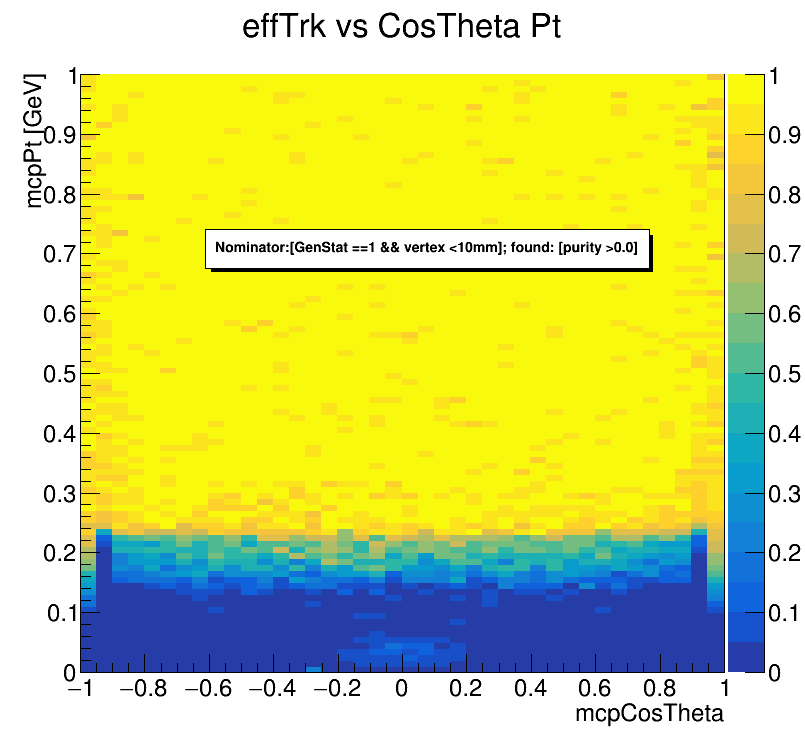
\includegraphics[width=0.5\hsize]{{Performance/fig/EffTrkPerformance2DcosThetaPt_purity0.0}.png} &
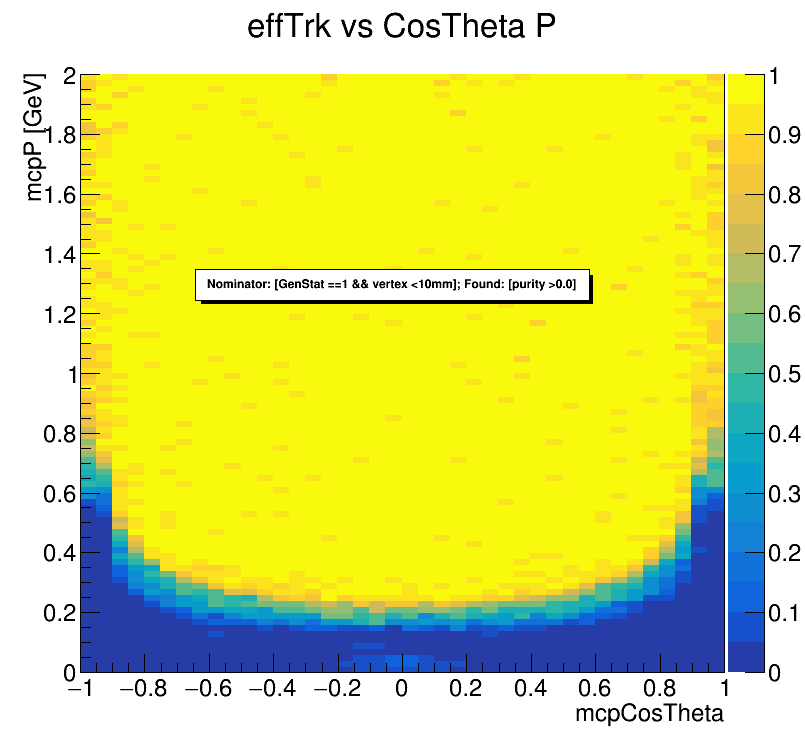
\includegraphics[width=0.5\hsize]{{Performance/fig/EffTrkPerformance2DcosThetaMomentum_purity0.0}.png}
\end{tabular}
\caption{\label{ild:fig:intro:tracking}Track finding efficiency for $t \bar t$-events at 500 GeV, as a function of transverse momentum (left),
  momentum (right) and $cos(\theta)$ for the large ILD detector model. }
\end{figure}



%
% tracking efficiency for single muons - 2D
% 
\thisfloatsetup{floatwidth=\SfigwFull,capposition=beside}
\begin{figure}[b!]
\begin{tabular}{cc}
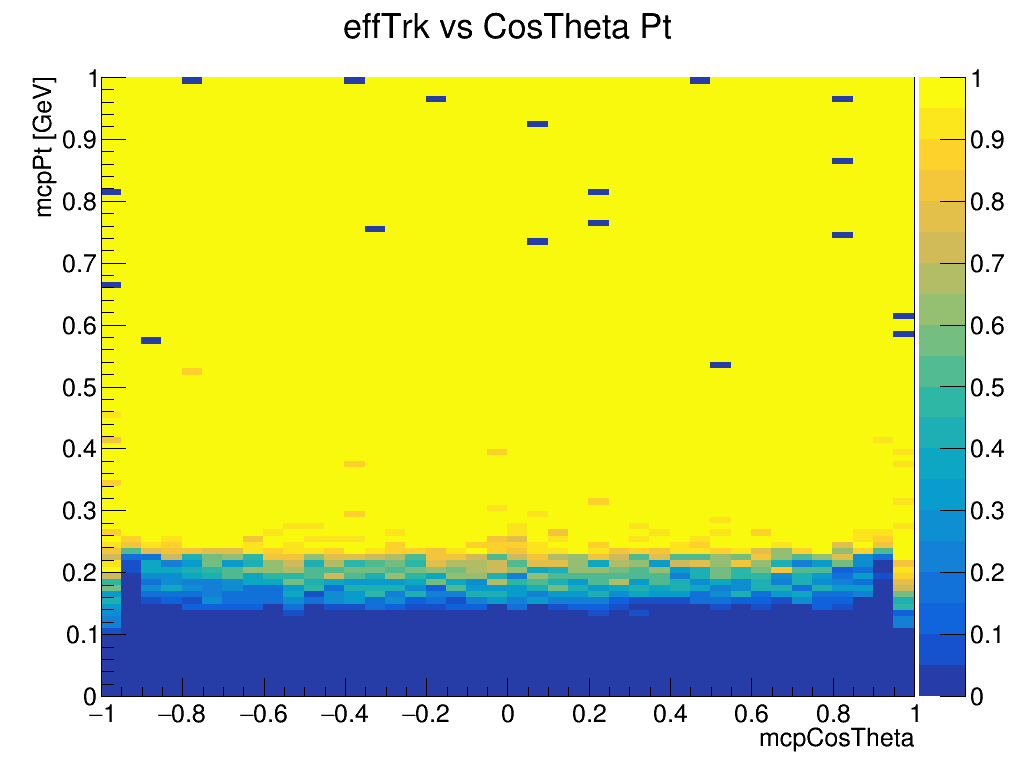
\includegraphics[width=0.5\hsize]{Performance/fig/SingleMuon_EffTrk2DCosThetaPt.png} &
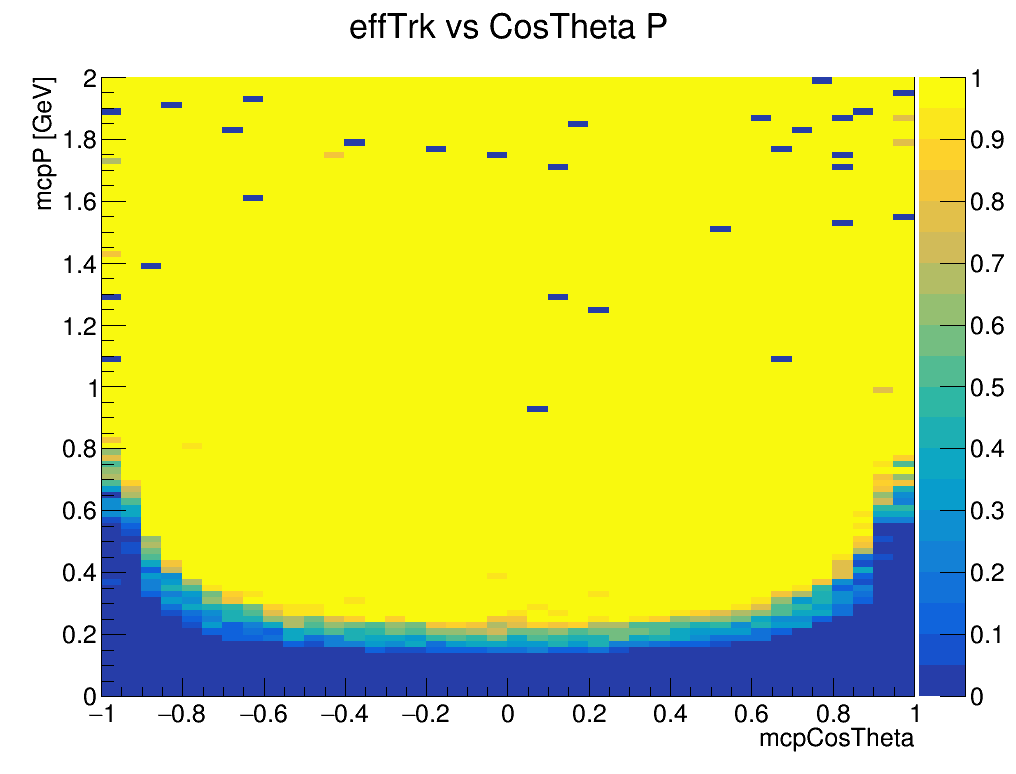
\includegraphics[width=0.5\hsize]{Performance/fig/SingleMuon_EffTrk2DCosThetaP.png}
\end{tabular}
\caption{\label{ild:fig:intro:tracking}Track finding efficiency for single muons as a function of transverse momentum (left),
  momentum (right) and $cos(\theta)$ for the large ILD detector model. \fix{FG: do we need these single particle eff. plots ?} }
 \end{figure}


\subsection{Particle Flow performance and JER}


%
% uds - JER w/ rms90 and JES
% 
\thisfloatsetup{floatwidth=\SfigwFull,capposition=beside}
\begin{figure}[b!]
\begin{tabular}{cc}
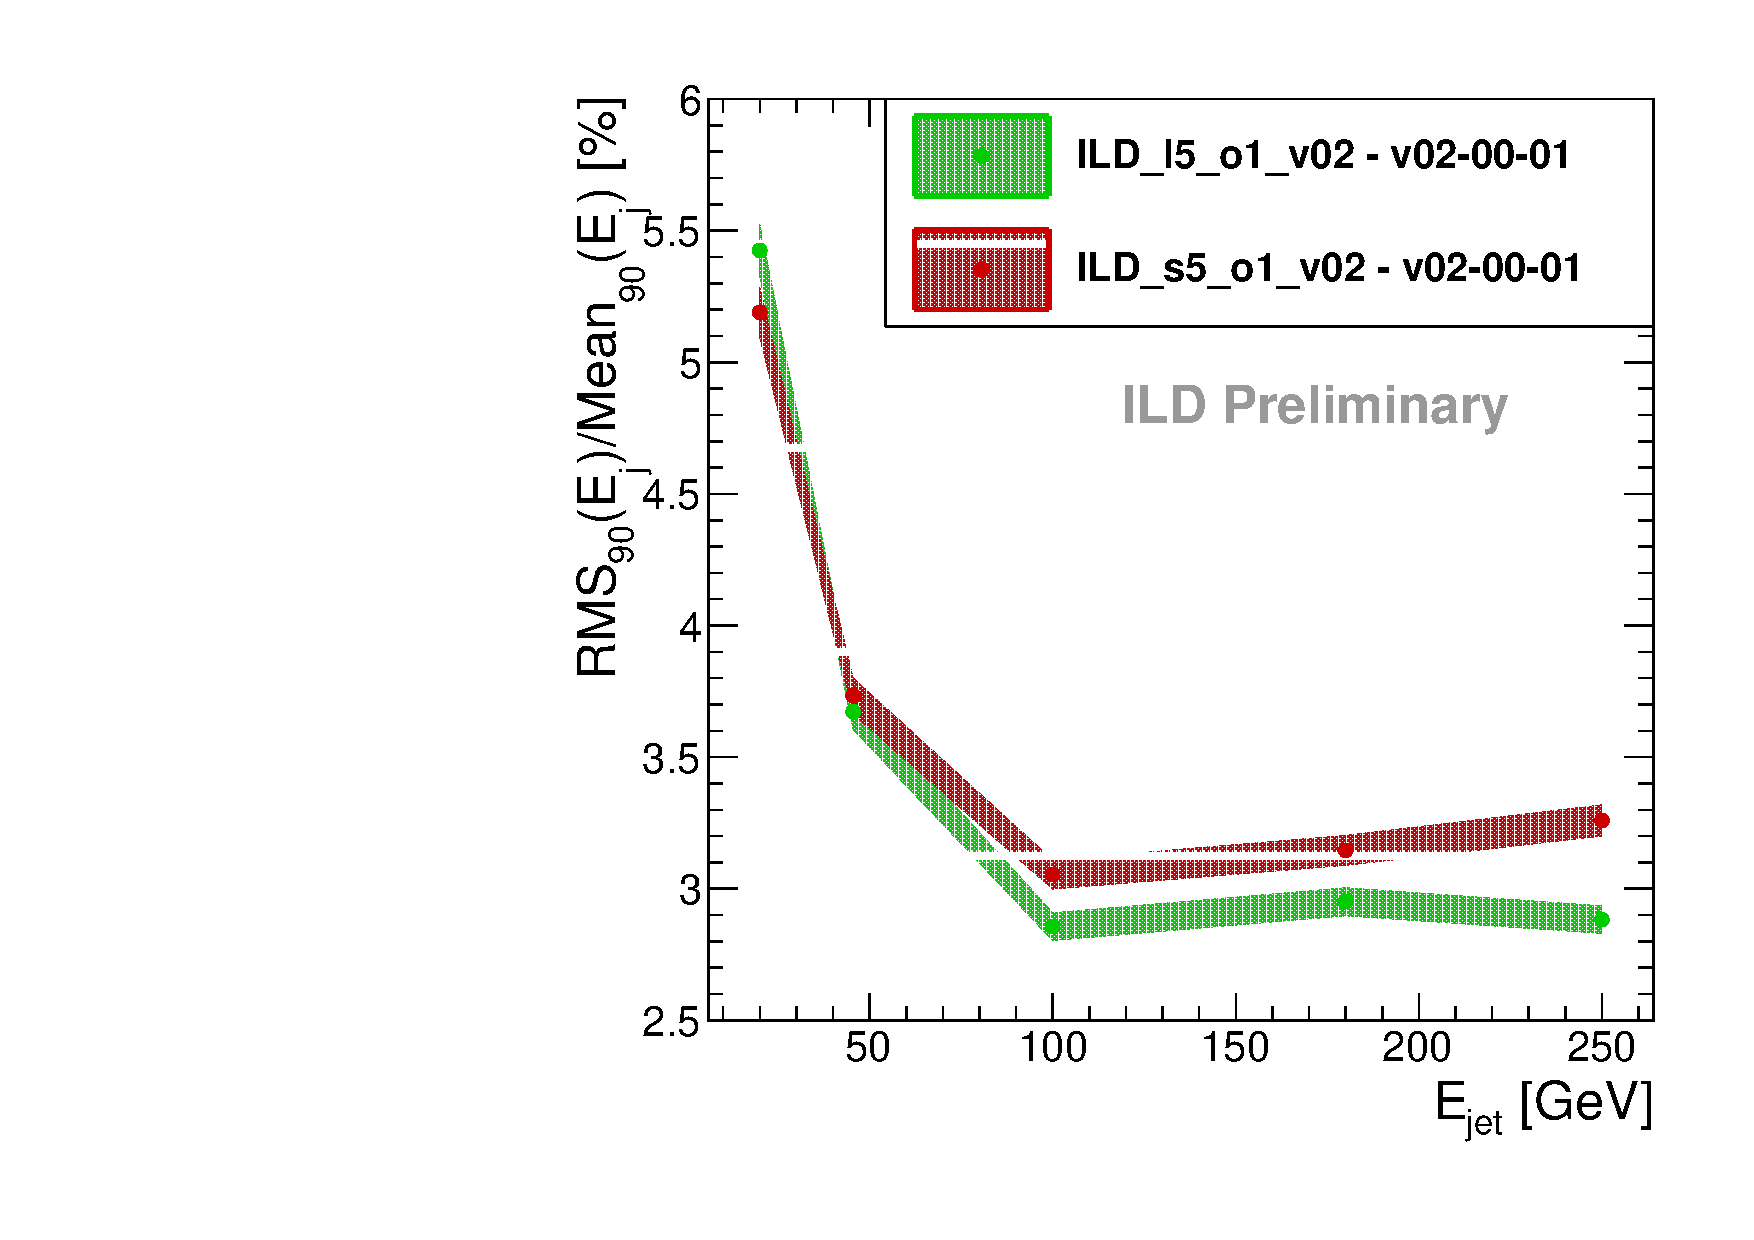
\includegraphics[width=0.5\hsize]{Performance/fig/JERLargeSmall_v02-00-01.pdf} &
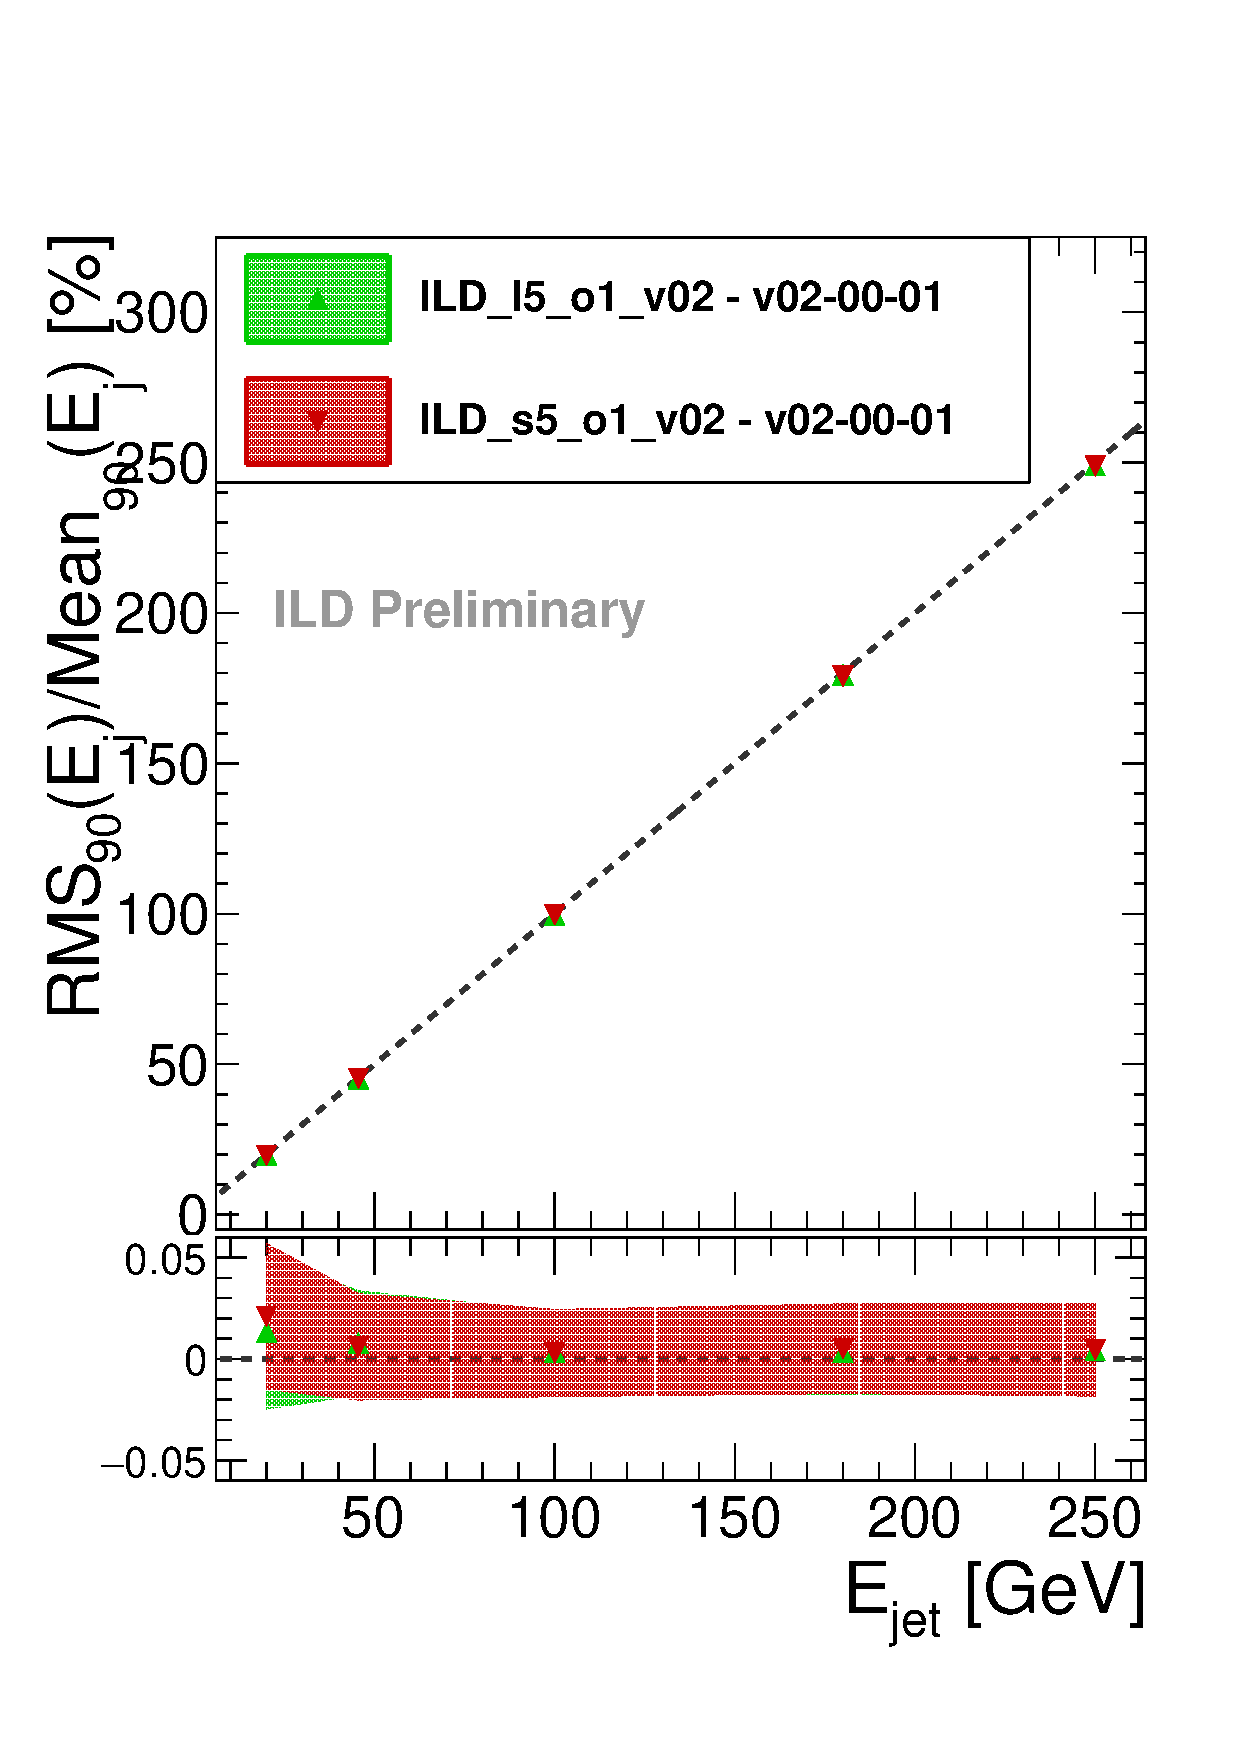
\includegraphics[width=0.5\hsize]{Performance/fig/JESLargeSmall_v02-00-01.pdf}
\end{tabular}
\caption{\label{ild:fig:intro:tracking} Jet energy resolution (left) and jet energy scale (right) for the large and small ILD detector
models as a function of the jet energy for uds di-jet events.}
 \end{figure}


%
% uds and bb/cc- JER w/ rms90 and JES
% 
\thisfloatsetup{floatwidth=\SfigwFull,capposition=beside}
\begin{figure}[b!]
\begin{tabular}{cc}
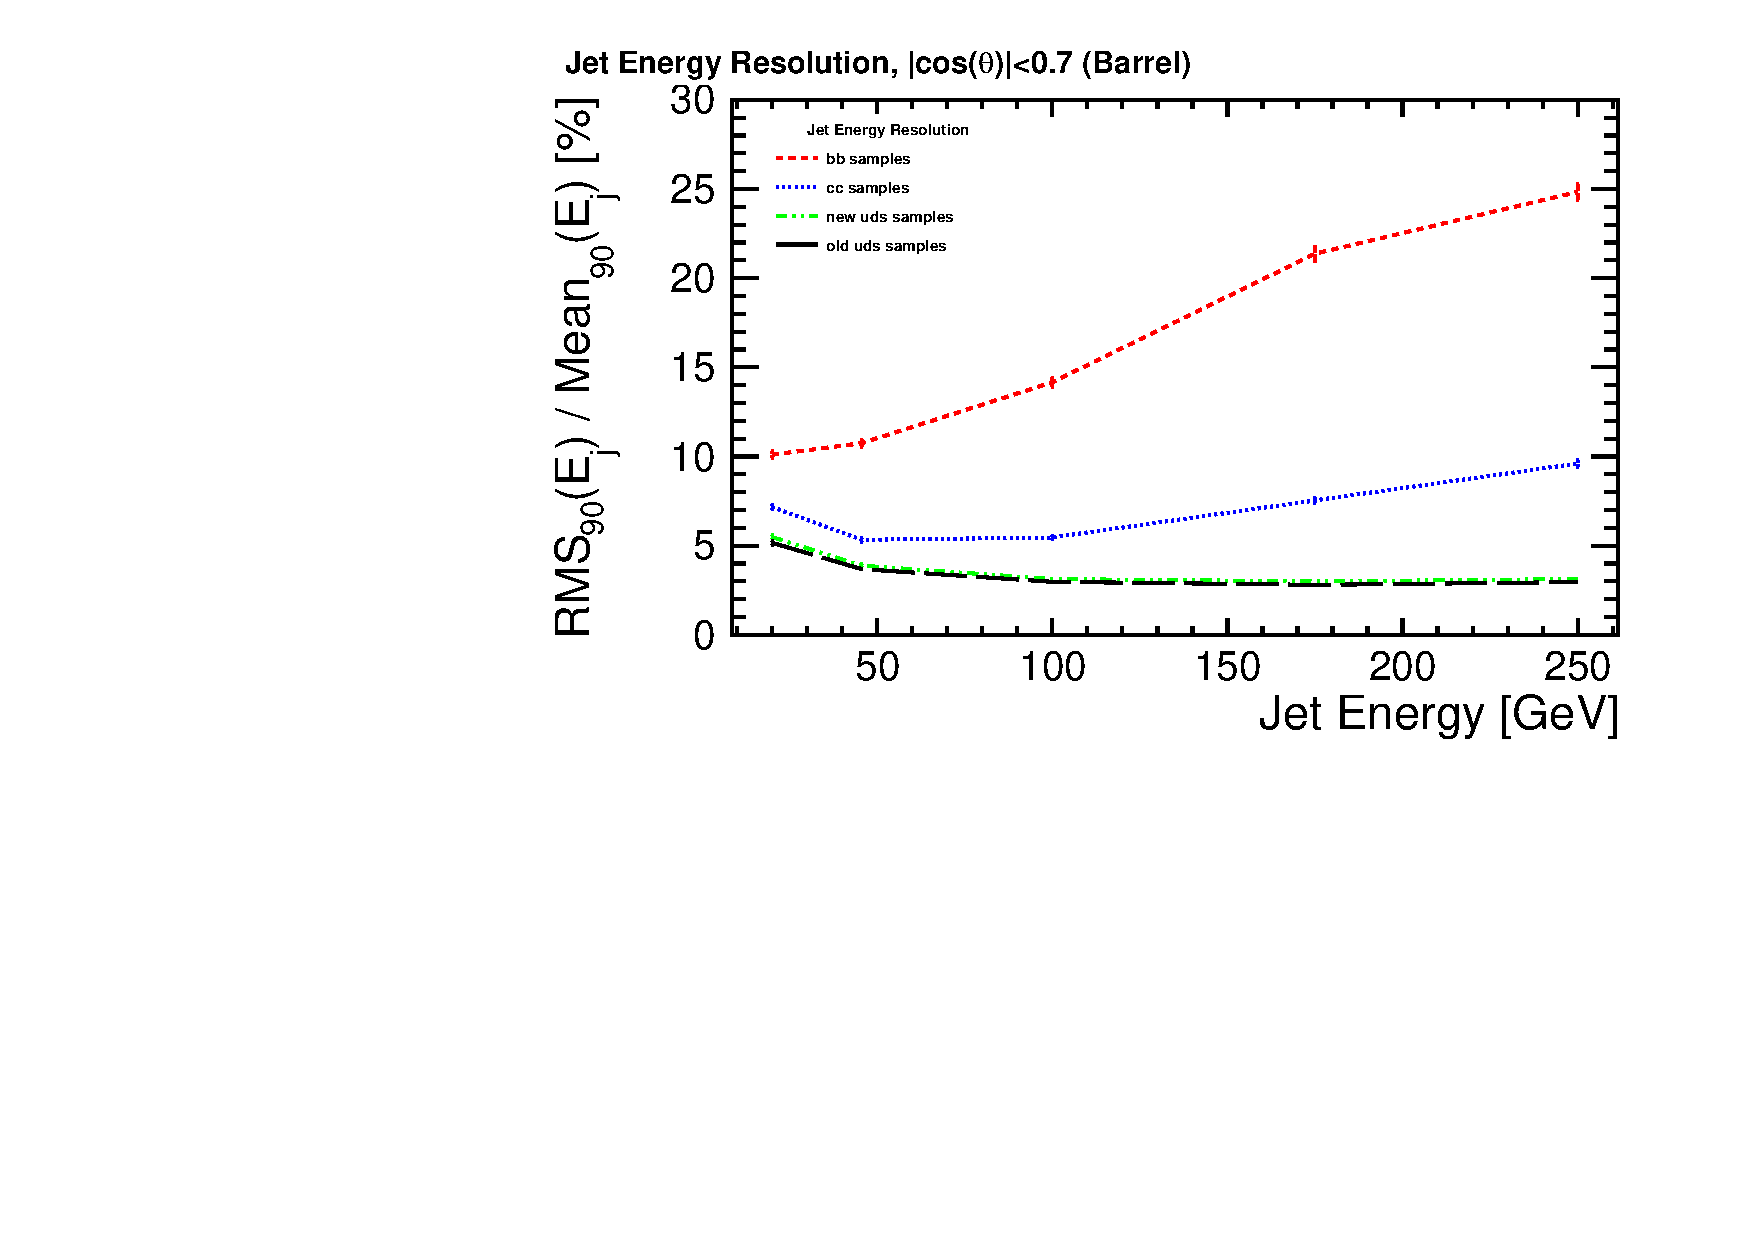
\includegraphics[width=0.5\hsize]{Performance/fig/Jet_Energy_Resolution_Barrel_new_cc_bb.pdf} &
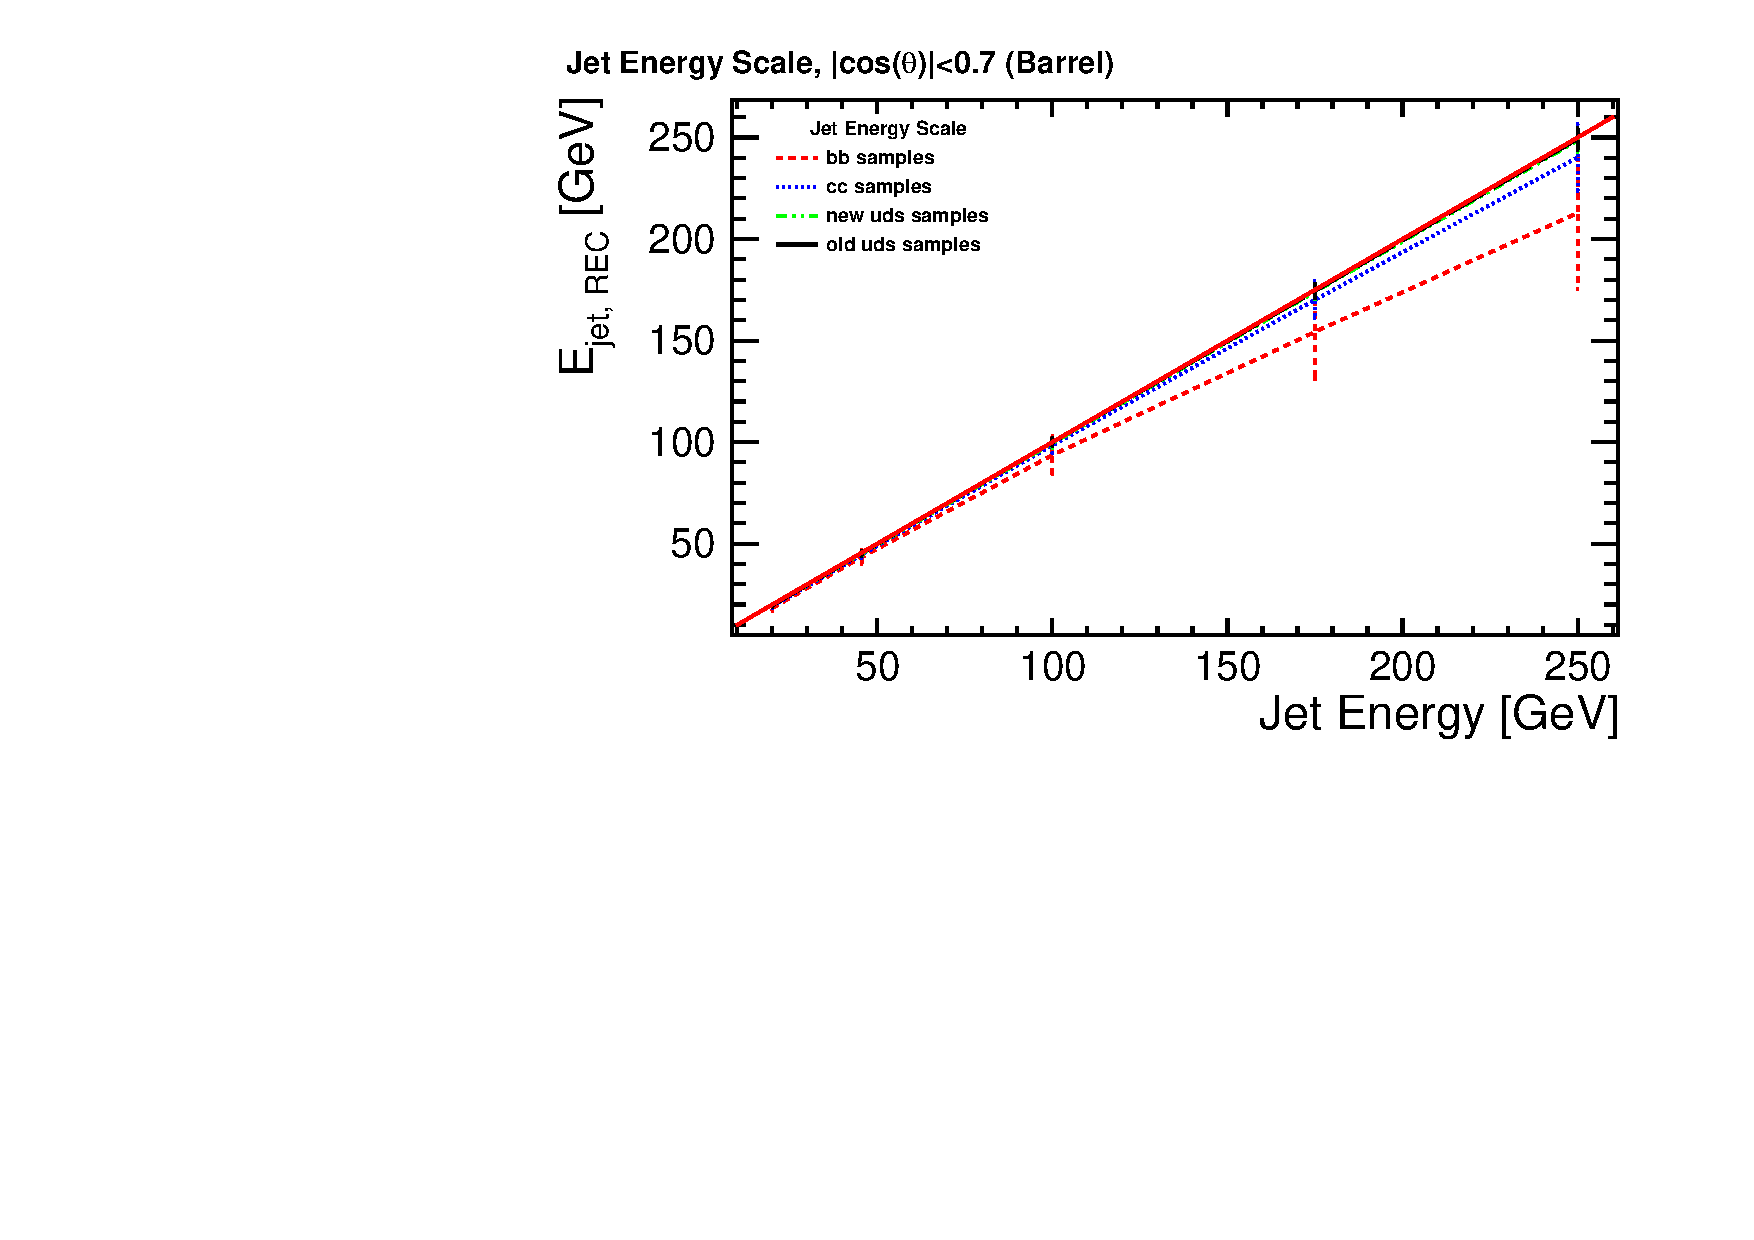
\includegraphics[width=0.5\hsize]{Performance/fig/Jet_Energy_Scale_Barrel_new_cc_bb.pdf}
\end{tabular}
\caption{\label{ild:fig:intro:tracking} Jet energy resolution (left) and jet energy scale (right) for cc and bb  as a function of the jet
  energy compared to uds events.}
 \end{figure}


\subsection{Photon Reconstruction}

\subsection{Lepton ID}
\fix{muons, electrons}

\subsection{Charged Particle identification}

\fix{dE/dx, potentially ToF, shower shapes}


%%%%%%%%%%%%%%%%%%%%%%%%%%%%%%%%%%%%%%%%%%%%%%%%%%%%%%%%%%%%%%%
\section{High-level Reconstruction Performance}

\writer{Graham Wilson, Frank Gaede, Jenny List}{5}
\subsection{neutral}
\subsection{hadronically decaying tau ID}
\subsection{V0 / in flight decays vs radius}
\subsection{Baryons / Meson recosntruction}
\fix{
\begin{itemize}
\item $\Lambda^+_c \to pK^- \pi^+$
\item $D^0$, $D^*$
\item $J\Psi \to \mu \mu$  / inclusive di-muon spectrum ?
\end{itemize}
}
\subsection{Di-jet mass resolution between Cambridge and full physics}
\begin{itemize}
\item $Z$ mass in $ZZ \to \nu\nu qq$, flavour separated
\item $W$ hadronic mass from $WW \to qq l\nu$
\item from Jakob $\nu\nu qqqq$
\item various levels of cheating with TrueJet
\end{itemize}


%%%%%%%%%%%%%%%%%%%%%%%%%%%%%%%%%%%%%%%%%%%%%%%%%%%%%%%%%%%%%%%%
\section{Physics Benchmarks}
\writer{Keisuke Fujii, Jenny List}{10}
\subsection{General Remarks}
\begin{itemize}
\item all benchmarks at 500\,GeV or even 1\,TeV since more challening for detector
\item Luminosity and polarisation according to H20 / running scenario paper: 
  \begin{itemize}
   \item 4\,ab$^{-1}$ at 500\,GeV, with $f(-+,+-,++,--) = (40\%,40\%, 10\%, 10\%)$
   \item 8\,ab$^{-1}$ at 1\,TeV, with $f(-+,+-,++,--) = (40\%,40\%, 10\%, 10\%)$.
\end{itemize}
\item benchmarks chosen to illustrate many performance aspects, not to cover complete physics case
\item analyses not optimised for utmost physics performance
\item in general DBD sample based analyses remain valid for physics
\item list of produced samples ?
\end{itemize}

%%%%%%%%%%%%%%%%%%%%%%%%%%%%%%%%%%%%%%%%%%%%%%%%%%%%%%%%%%%%%%%%%%%
\subsection{Hadronic Branching Ratios of the Higgs Boson}
\begin{itemize}
\item main physics observables: $\sigma(\nu\bar{\nu} H)\times BR(H\to b\bar{b} / c\bar{c} / gg)$
\item cross-section and/or generator level numbers ? 
\item brief analysis description: precuts, MVA, template fit
\item example MVA input: 
  \begin{itemize}
     \item reconstructed $M_H$ for large and small, signal and backgrounds. 
     \item possibly in addition also separately for $\nu\nu bb$ final state?
     \item and/or with cheated neutrinos in jets / perfect PFA / ...?
  \end{itemize}
\item example flavour tag: 
  \begin{itemize}
     \item full sim templates for $H \to bb / cc / gg$ (2D colz instead of lego?)
     \item cheated and artificially bad performance
  \end{itemize}
\end{itemize}

%%%%%%%%%%%%%%%%%%%%%%%%%%%%%%%%%%%%%%%%%%%%%%%%%%%%%%%%%%%%%%%%%%%
\subsection{Higgs Mass from $ZH \to ll b\bar{b}$}
%%%%%%%%%%%%%%%%%%%%%%%%%%%%%%%%%%%%%%%%%%%%%%%%%%%%%%%%%%%%%%%%%%%
\subsection{Branching Ratio of $H \to \mu^+\mu^-$}
\begin{itemize}
\item main physics observables: $\sigma(\nu\bar{\nu} H)\times BR(H\to \mu^+\mu^-)$
\item cross-section and/or generator level numbers  
\item brief analysis description: precuts, MVA, toy MC fit to mass distribution
\item example variables: 
  \begin{itemize}
     \item event-by-event Higgs mass resolution (l5 / s5)
     \item reconstructed $M_H$ for large and small, signal and backgrounds
   
     \item cheated muons / ISR / ?
  \end{itemize}
\item BR precision vs momentum resolution: 
  \begin{itemize}
     \item full sim results s5 /l5
     \item on cheated and smeared...
  \end{itemize}
\end{itemize}

%%%%%%%%%%%%%%%%%%%%%%%%%%%%%%%%%%%%%%%%%%%%%%%%%%%%%%%%%%%%%%%%%%%
\subsection{Sensitivity to $H \to $ invisible}
\begin{itemize}
\item main physics observables: $\sigma(q\bar{q} H)\times BR(H \to \mbox{inv.})$
\item cross-section and/or generator level numbers 
\item brief analysis description: precuts, MVA, limit setting
\item example variables:
  \begin{itemize}
     \item reconstructed $M_Z \to q\bar{q}$ and recoil mass for large and small, signal      \item in addition also separately for each jet flavour ?
     \item and/or with cheated neutrinos in jets / perfect PFA / cheated ISR...?
  \end{itemize}
\item results: 
  \begin{itemize}
     \item full sim limit
     \item limit vs JER
  \end{itemize}
\end{itemize}

%%%%%%%%%%%%%%%%%%%%%%%%%%%%%%%%%%%%%%%%%%%%%%%%%%%%%%%%%%%%%%%%%%%
\subsection{$\tau$ decay modes and polarisation, $A_{FB}$ and $A_{LR}$ in $e^+e^- \to \tau^+\tau^-$}
%%%%%%%%%%%%%%%%%%%%%%%%%%%%%%%%%%%%%%%%%%%%%%%%%%%%%%%%%%%%%%%%%%%
\subsection{$W$ mass, Triple Gauge Couplings and Beam Polarisation from $e^+e^- \to WW \to qql\nu$}
%%%%%%%%%%%%%%%%%%%%%%%%%%%%%%%%%%%%%%%%%%%%%%%%%%%%%%%%%%%%%%%%%%%
\subsection{Quartic Gauge Couplings in $e^+e^- \to \nu\nu qqqq$}
%%%%%%%%%%%%%%%%%%%%%%%%%%%%%%%%%%%%%%%%%%%%%%%%%%%%%%%%%%%%%%%%%%%
\subsection{$A_{LR}$ and Jet Energy Scale Calibration from $e^+e^- \to \gamma Z$}
%%%%%%%%%%%%%%%%%%%%%%%%%%%%%%%%%%%%%%%%%%%%%%%%%%%%%%%%%%%%%%%%%%%
\subsection{$A_{FB}$ and $A_{LR}$ from $tt \to bb qqqq$}
%%%%%%%%%%%%%%%%%%%%%%%%%%%%%%%%%%%%%%%%%%%%%%%%%%%%%%%%%%%%%%%%%%%
\subsection{Discovery Reach for extra Higgs Bosons in $e^+e^- \to Zh$}
%%%%%%%%%%%%%%%%%%%%%%%%%%%%%%%%%%%%%%%%%%%%%%%%%%%%%%%%%%%%%%%%%%%
\subsection{Discovery Reach for and Characterisation of low $\Delta M$ Higgsinos}
%%%%%%%%%%%%%%%%%%%%%%%%%%%%%%%%%%%%%%%%%%%%%%%%%%%%%%%%%%%%%%%%%%%
\subsection{WIMP Discovery Reach and Characterisation in the Mono-Photon Channel}

